\documentclass[a4paper, 12pt]{article}

% --- Пакеты для русского языка ---
\usepackage[T2A]{fontenc}
\usepackage[utf8]{inputenc}
\usepackage[russian]{babel}

% --- Математические пакеты ---
\usepackage{amsmath}
\usepackage{amssymb}
\usepackage{amsfonts}

% --- Пакет для изображений ---
\usepackage{graphicx}

% --- Настройка полей страницы ---
\usepackage[left=2cm, right=2cm, top=2.5cm, bottom=2.5cm]{geometry}

% --- Настройка межстрочного интервала ---
\usepackage{setspace}
\onehalfspacing % Полуторный интервал

\title{Конспект по теории шумов}
\author{Лекция 1}
\date{} % Убираем дату

\begin{document}
\begin{titlepage}
    \vspace*{\fill} % Заполняем вертикальное пространство сверху
    \begin{center}
        \Huge \textbf{Шумы в электронных цепях} \\
        \vspace{1cm} % Добавляем вертикальный отступ
        \large (конспект семинара)
    \end{center}
    \vspace*{\fill} % Заполняем вертикальное пространство снизу
\end{titlepage}
\pagebreak % Начинаем текст лекции с новой страницы
% \maketitle % Можете раскомментировать, если хотите титульный лист

\section{Вступление}
Каждый, кто хоть раз работал с осциллографом или вольтметром замечал, что напряжение или сила тока в цепи никогда не принимают строго определенное значение, они постоянно меняются, "пляшут" вокруг некоторой величины. Это так называемые \textbf{шумы} или флуктуации, которые присутствуют в цепях, как и в любых других физических системах. Для описания шумов нам понадобится математический аппарат теории вероятностей, так как шум представляет собой случайный процесс, поэтому будет разумно для начала вспомнить необходимую математическую теорию.

\section{Необходимые знания из теории вероятностей}
\subsection{Характеристики случайной величины}
\textbf{Случайная величина} — это переменная, которая в результате случайного эксперимента принимает одно из множества возможных числовых значений. Мы не можем предсказать точное значение, которое она примет, но можем описать вероятность появления тех или иных значений. Далее мы будем говорить о непрерывных случайных величинах. Случайная величина полностью описывается своей плотностью вероятности $f(x)$.

\textbf{Математическое ожидание} - характеристика случайной величины , которая определяется формулой:
$$
E[X] = \int\limits_{-\infty}^{\infty}x f(x)dx
$$
Математическое ожидание имеет смысл среднего взвешенного.

\textbf{Дисперсия} определяется через математическое ожидание:
$$
D[X] = E[(X - E[X])^2]
$$
Дисперсия является мерой разброса случайной величины. Можно переписать в другом виде:
$$
D[X] = E[X^2] -E^2[X] 
$$
Иногда это бывает полезно.
Дисперсия имеет размерность квадрата величины, поэтому иногда бывает удобнее пользоваться \textbf{среднеквадратичным отклонением}:
$$
\sigma_X = \sqrt{D[X]}
$$

\subsection{Независимость}
События $A$ и $B$ называются \textbf{независимыми}, если для их математических ожиданий выполняется следующее тождество:
$$
P[AB] = P[A]P[B]
$$
Однако более интуитивное определение получится, если переписать это выражение:
$$
P[A] = P[A|B] = \frac{P[AB]}{P[B]}; \qquad P[B]= P[B|A] = \frac{P[AB]}{P[A]}
$$
Получаем определение условной вероятности. Отсюда видно, что случайные величины независимы, если информация о значении одной из них не дает дополнительной информации о величине другой. 

\subsection{Ковариация}
\textbf{Ковариация} случайной величины определяется следующей формулой:
$$
\text{cov}(X, Y) = E[(X - E[X])(Y - E[Y])] = E[XY] - E[X]E[Y]
$$
Ковариация показывает, насколько синхронно изменяются две величины, если ковариация равна нулю, величины называют некоррелированными.(не путать с независимостью!). \textbf{Коэффициент корреляции} представляет из себя нормированную ковариацию:
$$
\rho_{XY} = \frac{\text{cov}(X,Y)}{\sigma_X\sigma_Y} \in [-1, 1]
$$

\subsection{Случайный процесс}
Теперь поговорим об основном объекте нашего исследования.
\textbf{Случайный процесс} $X(t, \omega)$ - это функция двух переменных:
\begin{enumerate}
    \item t (Обычно время) - аргумент из некоторого множества $T$.
    \item Элементарного исхода $\omega$, принадлежащего пространству элементарных исходов $\Omega$. 
\end{enumerate}

Представьте себе завод по производству генераторов шума. Возьмем все произведенные на заводе генераторы и одновременно включим их. Аргумент $\omega$ отвечает за выбор генератора шума, а $t$ за выбор момента времени, в который мы смотрим на значение генератора. То есть конкретный генератор символизирует реализацию случайного процесса, которая является функцией времени. Если мы фиксируем время и смотрим значения на разных генераторах, то получаем случайную величину. 

% --- МЕСТО ДЛЯ ВАШЕГО ИЗОБРАЖЕНИЯ ---
\begin{figure}[h!]
    \centering
    % Раскомментируйте следующую строку и убедитесь, что
    % файл 'generators.png' находится в той же папке:
    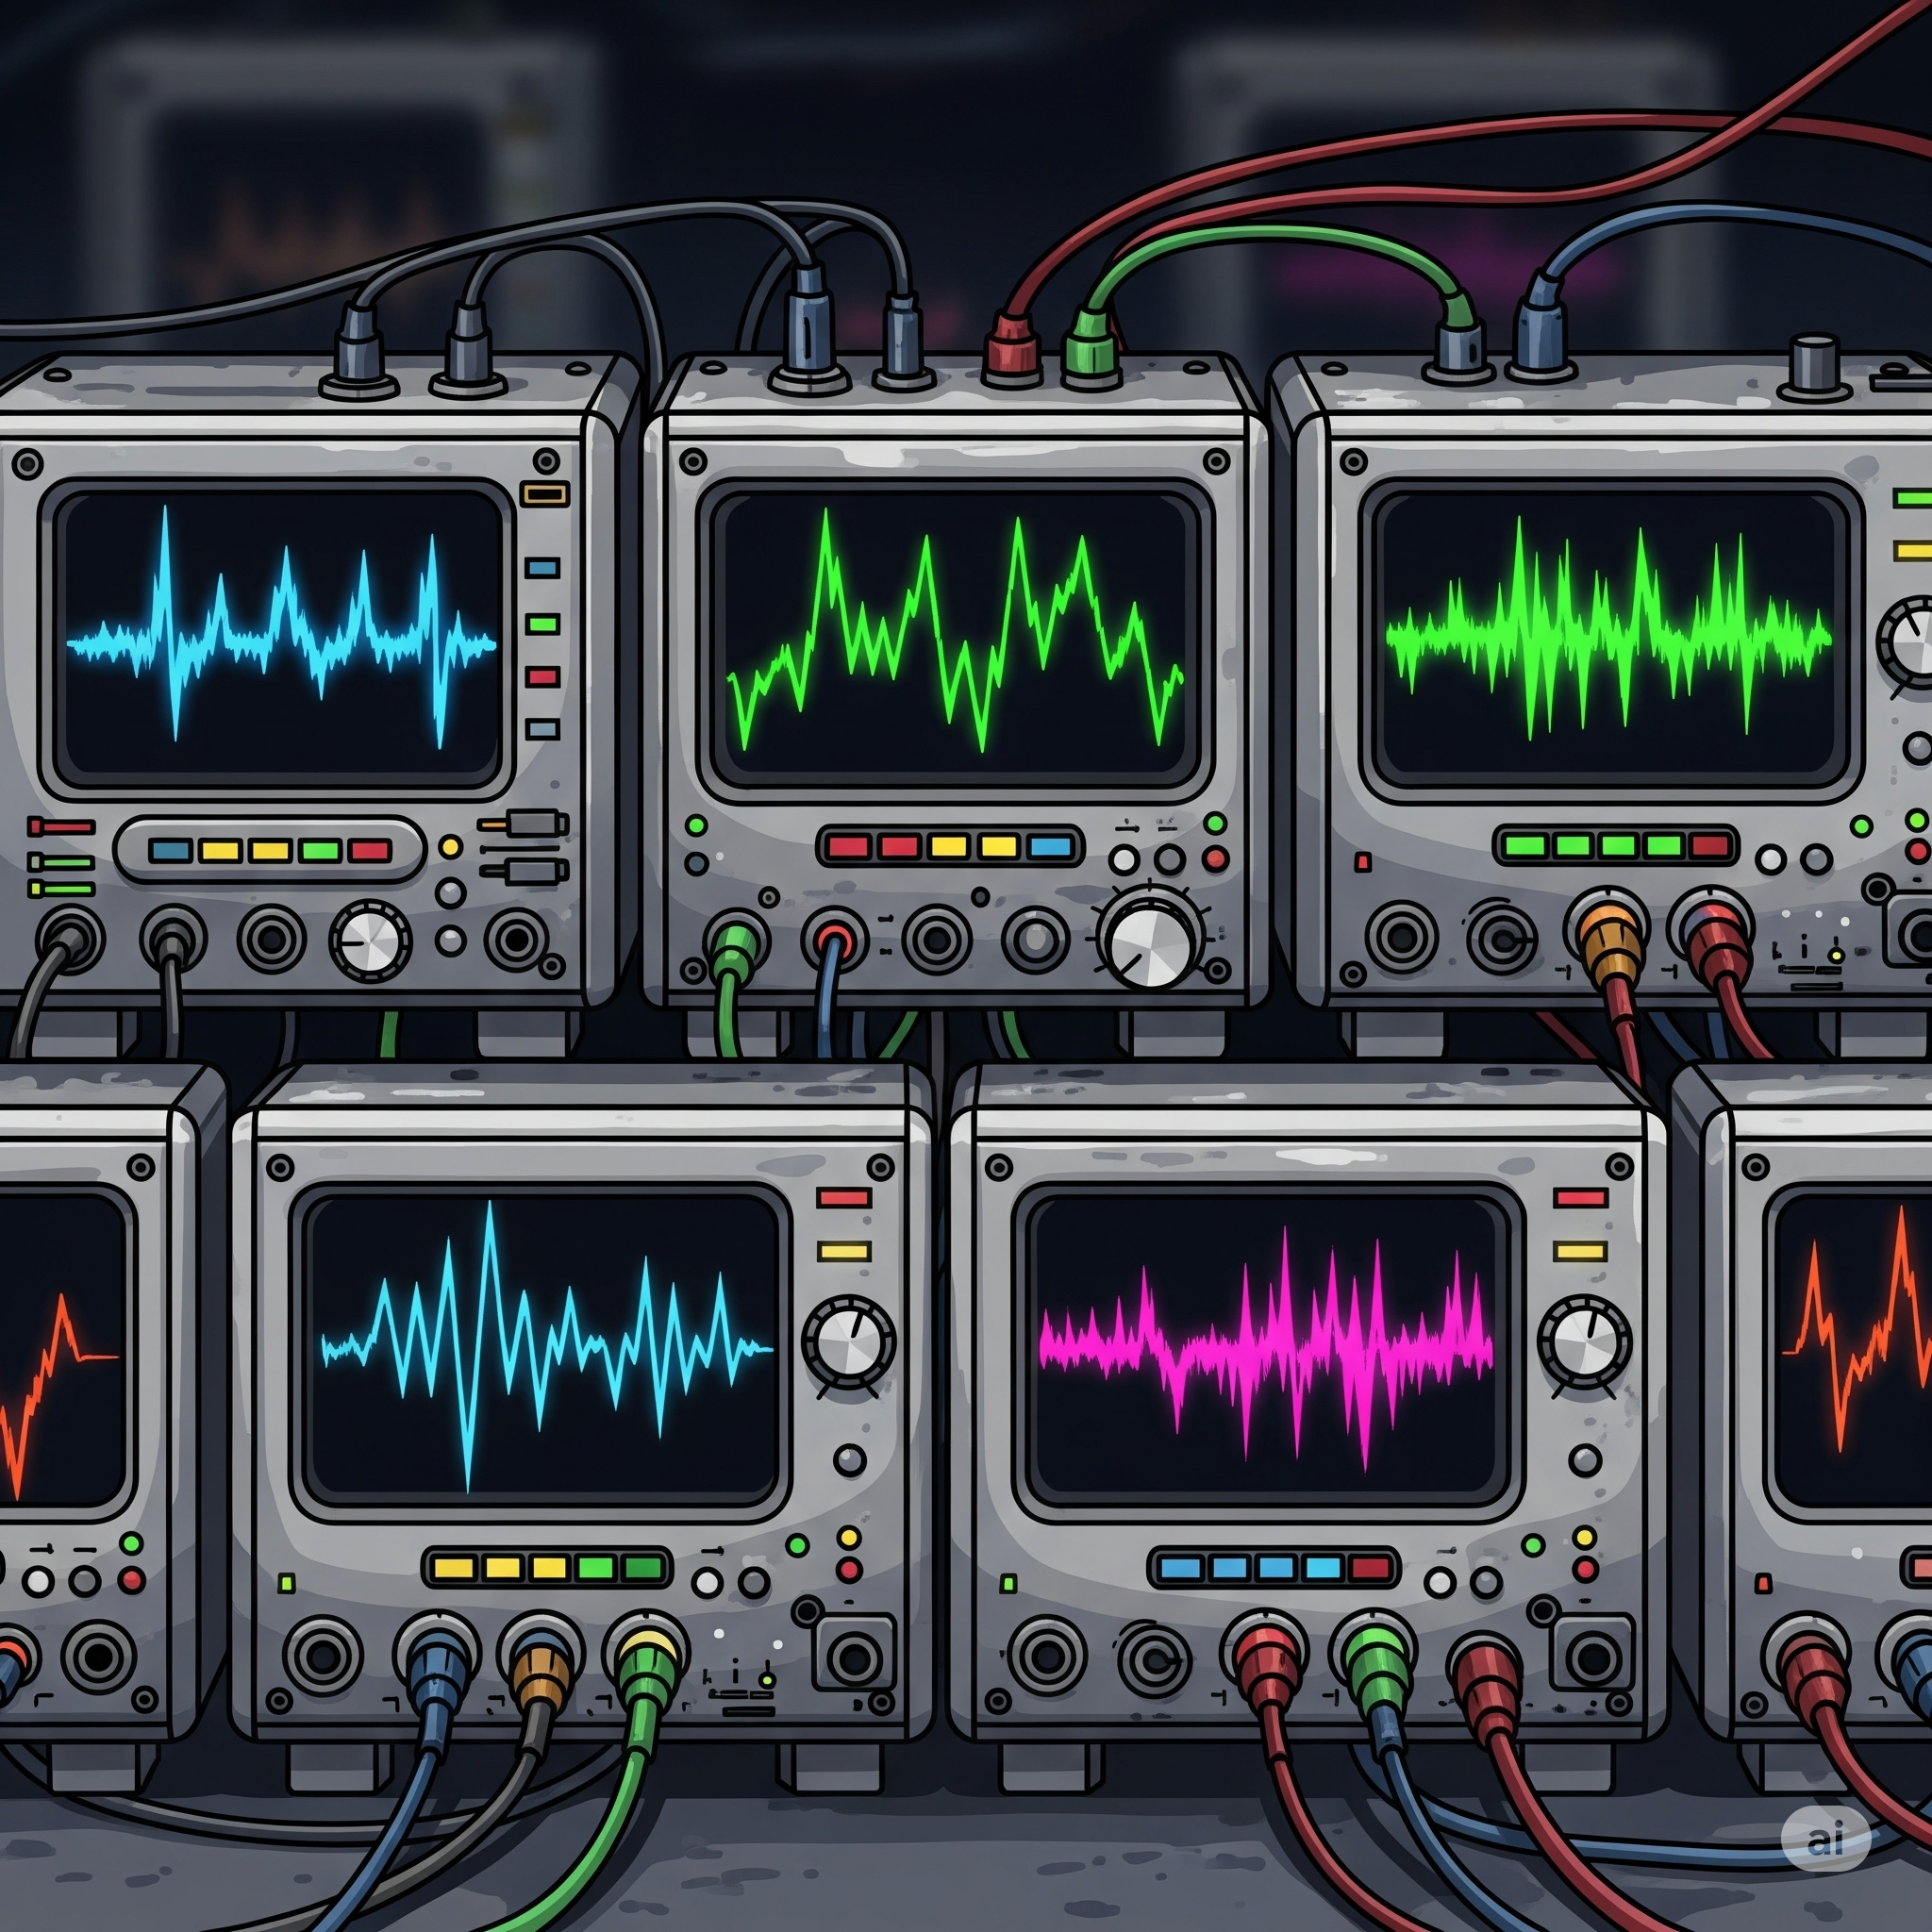
\includegraphics[width=0.4\textwidth]{Images/generators.png}
    % Временный плейсхолдер:
    \caption{Иллюстрация ансамбля случайных процессов.}
    \label{fig:generators}
\end{figure}
% ---------------------------------

Здесь стоит сделать важное замечание. Далее мы будем рассматривать только \textbf{эргодические} случайные процессы. Все реальные шумы относятся к этому классу. Процесс называется эргодическим, если усреднение по времени одной единственной реализации дает тот же результат, что и усреднение по всему ансамблю в один момент времени. То есть если мы возьмем один единственный генератор шума с нашего завода и вычислим среднее, то получим тот же результат, как если бы усредняли по значениям всех генераторов в фиксированный момент времени.

Эргодический процесс всегда является также и стационарным. Это значит, что его вероятностные характеристики не зависят от времени. Разница между стационарностью и эргодичностью хоть и не велика, но присутствует. Не каждый стационарный процесс является эргодическим. 

Если мы хотим вычислить математическое ожидание или дисперсию для стационарного процесса, мы можем просто зафиксировать произвольный момент вычислить их через формулу для случайной величины. Плотность вероятности в силу стационарности не зависит от времени.
$$
E[x] = \int x \rho(x)dx
$$

Если же процесс является эргодическим, то вычисление вероятностных характеристик сводится к "усреднению по времени":
$$
E[x] = \lim\limits_{T\rightarrow\infty} \frac{1}{2T}\int\limits_{-T}^{T}x(t)dt \qquad D[x] = \lim\limits_{T\rightarrow\infty} \frac{1}{2T}\int\limits_{-T}^{T}[x(t)-E[x]]^2dt
$$

Для случайных процессов также вводится корреляция. 
Если присутствует два случайных процесса, то рассматривается \textbf{взаимная корреляционная функция}:
$$
\langle x, y \rangle (\tau) = E\left[ x(u)y(u-\tau) \right]
$$
Для одного сигнала рассматривается \textbf{автокорреляция}:
$$
\langle x, x \rangle (\tau) = E\left[ x(u)x(u-\tau) \right]
$$
Пользуясь эргодичностью можно аналогично математическому ожиданию и дисперсии заменить усреднение по выборкам на усреднение по времени отдельной реализации:
$$
\langle x, y \rangle (\tau) = \lim\limits_{T \rightarrow\infty}\frac{1}{T}\int\limits_{-T/2}^{T/2}x(u)y(u-\tau)du
$$
(И аналогично для автокорреляции)
Заметим схожесть формулы автокорреляции с формулой свертки, (отличие лишь в порядке $u-t$, поэтому для корреляции коммутативность в отличие от свертки не выполняется).

Теперь мы готовы к изучению теории шумов.

\section{Шум}
Шум $n(t)$ является эргодическим, а значит стационарным случайным процессом. Тогда можно вычислять вероятностные характеристики аналогично вычислению характеристик случайных величин. Мощностью шума называется следующее выражение:
$$
\sigma^2 = E[n^2] = \int n^2 p(n)dn
$$
где $p(n)$ - плотность распределения. Такое обозначение шума введено для того, чтобы сам символ $\sigma$ обозначал \textbf{эффективное значение шума}.
Пользуясь эргодичностью сведем вычисление мощности к интегрированию по времени.
$$
\sigma_T^2 = \frac{1}{T}\int\limits^{T/2}_{-T/2}n^2(u)du \approx \frac{1}{N}\sum\limits_{i=1}^N n^2(u_i)
$$
Таким образом можно вычислить приблизительное значение мощности экспериментально. Автокорреляцию шума называют просто \textbf{корреляцией шума} и обозначают таким символом:
$$
n^2(t) = \langle n, n \rangle (t) = E[n(u)n(t-u)]
$$
Заметим, что при $t = 0$ корреляция шума равна его мощности.

Для нескольких шумов вводится понятие взаимной корреляции, которое полностью совпадает с взаимной корреляцией случайных процессов:
$$
\langle n_1, n_2 \rangle (t) = \lim\limits_{T \rightarrow\infty}\int\limits_{-T/2}^{T/2}n_1(u)n_2(u-t)du
$$
\textbf{Важно!} Шум является эргодическим случайным процессом. Это значит, что его вероятностные характеристики не зависят от абсолютного времени. Следовательно корреляция - это вполне определенная функция! (Также как матожидание и дисперсия у случайных величин.) Значит эта функция как-то характеризует шум.

Шумы называются \textbf{некоррелированными}, если их взаимная корреляция тождественно равна нулю:
$$
\langle n_1, n_2 \rangle (t) \equiv 0
$$
Далее мы будем считать, что все шумы, порожденные разными физическими механизмами некоррелированны. (Умная фраза из Григорьева. ну а с чего бы им быть коррелированными)

\section{Спектральная плотность шума}
Это каноническая (математическая) форма прямого и обратного преобразований Фурье.
$$
\mathcal{F}\left[x\right](\omega) = \text{v.p.}\frac{1}{\sqrt{2\pi}}\int\limits_{-\infty}^{\infty}x(t)e^{-i\omega t} dt; \qquad 
\mathcal{F}^{-1}\left[X\right](t) = \text{v.p.}\frac{1}{\sqrt{2\pi}}\int\limits_{-\infty}^{\infty}X(\omega)e^{+i\omega t} d\omega
$$
% Примечание: В исходном тексте в обратном Фурье было X(t), исправлено на X(\omega)
Спектральная плотность шума $n^2(f)$ определяется следующим образом:
$$
\frac{n^2(f)}{2} =\int\limits_{-\infty}^{\infty}n^2(t)e^{-j2\pi ft} dt 
$$
По сути спектральная плотность шума это \textbf{преобразование Фурье} от корреляции шума. Однако форма записи несколько отличается, поэтому для ясности последовательно перейдем от канонической формы к определению $n^2(t)$. 
Обычно в физике в отличие от математики преобразование Фурье определяют несколько иначе, перенося коэффициент $\frac{1}{\sqrt{2 \pi}}$ из прямого преобразования в обратное. А также опускают $\text{v.p.}$
$$
\mathcal{F}\left[x\right](\omega) = \int\limits_{-\infty}^{\infty}x(t)e^{-i\omega t} dt; \qquad 
\mathcal{F}^{-1}\left[X\right](t) = \frac{1}{2\pi}\int\limits_{-\infty}^{\infty}X(\omega)e^{+i \omega t} d\omega
$$
Теперь перейдем от угловой частоты к обычной частоте, измеряемой в Герцах: $\omega = 2 \pi \nu$. При этом изменится и дифференциал: $d\omega = 2\pi d\nu$. Видим, что $2\pi$ сократятся.

$$
\mathcal{F}\left[x\right](\nu) = \int\limits_{-\infty}^{\infty}x(t)e^{-i2\pi \nu t} dt; \qquad 
\mathcal{F}^{-1}\left[X\right](t) =\int\limits_{-\infty}^{\infty}X(\nu)e^{+i2\pi\nu t} d\nu
$$

Осталось обсудить двойку в знаменателе.
Если мы посмотрим на определение корреляции шума $n^2(t)$ то увидим, что это четная действительная функция. Как известно в таком случае Фурье образ также будет вещественной четной функцией. 

$$
\int\limits_{-\infty}^{\infty}n^2(t)e^{-j2\pi ft} dt = \int\limits_{-\infty}^{\infty}n^2(t)(\cos(-2\pi ft) + j\sin(-2\pi ft))dt
$$
% Примечание: В исходном тексте была опечатка \cos(-j2\pi ft)
Если спектр является четной функцией, значит ее отрицательная ось частот не несет в себе информации. Таким образом ее можно отбросить. Однако для сохранения мощности стоит удвоить положительную часть. В этом и кроется смысл удвоения: $n^2(f)$ - это \textbf{односторонняя} плотность, которая во всех точках вдвое больше исходной плотности.

Корреляцию, как обратное преобразование Фурье можно выразить через спектральную плотность шума:

$$
n^2(t) = \int\limits_{-\infty}^{+\infty} \frac{n^2(f)}{2}e^{+j2\pi ft}d f
$$
Опять же отметим, что спектральная плотность шума - это тоже вполне определенная функция, а значит может характеризовать шум.

\subsection{Размерности}
Какую размерность имеет $n^2(t)?$ Если сигнал, который мы наблюдаем измеряется в вольтах, то из определения можно увидеть, что корреляция шума имеет размерность $[V^2]$. Двойка в символе корреляции как раз указывает на квадратичность. Заметим таким образом, что корреляция пропорциональна мощности сигнала, которая имеет размерность $\left[\frac{V^2}{R}\right]$. Спектральная плотность определяется через интеграл корреляции по времени, ее размерность $[V^2 T]$, а значит спектральная плотность пропорциональна энергии. 

\subsection{Путаница определений}
Вместо спектральной плотности иногда используют корень из спектральной плотности.
$$
n(f) = \sqrt{n^2(f)} 
$$
Он уже имеет размерность $\left[V\sqrt{T}\right]$, поэтому называется эффективным значением спектральной плотности шума (напряжения/тока). Название довольно длинное, поэтому его сокращают до "шумового напряжения " (или шумовой тока) , и это порождает путаницу. Нужно уметь различать эти понятия.
Также эффективное напряжение шума $\sigma = \sqrt{\sigma^2}$ называют \textbf{напряжением шума}, но лучше согласно методичке называть это \textbf{уровнем шума}.

\end{document}